\chapter{Electronic spins in Diamond}

Lorem ipsum dolor sit amet, consectetur adipisicing elit, sed do eiusmod
tempor incididunt ut labore et dolore magna aliqua. Ut enim ad minim veniam,
quis nostrud exercitation ullamco laboris nisi ut aliquip ex ea commodo
consequat. Duis aute irure dolor in reprehenderit in voluptate velit esse
cillum dolore eu fugiat nulla pariatur. Excepteur sint occaecat cupidatat non
proident, sunt in culpa qui officia deserunt mollit anim id est laborum.
%TODO_MAR:  Status: Up for revision
% TODO_MAR: Fix definition of weakly coupled carbons
\section{Spin Control}
\label{controlingspinsindiamond}

% TODO_MAR: Rewrite introduction of diamond spin control chapter

The Nitrogen Vacancy centre in diamond is a well investigated system~\citep{Doherty2013NitrogenVacancy} and a promising candidate for quantum computation \citep{Childress2013Diamond}. In order to implement three qubit measurement based QEC we need three qubits plus ancillae that we can initialise, measure and conditionally perform operations on. These extra qubits are found in Carbon--13 atoms, which are normally a source of decoherence. These atoms can be addressed using a resonant decoupling sequence~\citep{Taminiau2012Detectiona}.

It has been shown that the nuclear- and electron- spin-state of the NV- centre can be initialized, coherently controlled and read-out using microwaves and laser pulses~\citep{Robledo2011HighFidelity}. These are essential tools in controlling the NV- centre. In this chapter I will explain how control over the electron-spin-state can be used to address weakly coupled Carbon--13 atoms.

\subsection{Spin Control}
\label{spincontrol}

The electronic ground state Hamiltonian can be written as~\citep{Pfaff2013Quantum}:
 \begin{equation}
H_{GS} = \Delta {S_z}^2 + \gamma_e \mathbf{B} \cdot \mathbf{S}
\end{equation}

With zero field splitting $\Delta \approx 2.88 \mathrm{GHz}$  and gyromagnetic ratio $\gamma_e  = 2.802$ MHz/G . In this expression the interactions with the Nitrogen nucleus and the Carbon spin bath are not included. By applying a magnetic field $B_z$ a long the N-V axis the degeneracy of the  $m_s =\pm1$ states is lifted by the Zeeman effect. A two level system that serves as a qubit can be defined with  $m_s=0:=|0\rangle$ and $m_s = -1 := |1\rangle$.

On the bloch-sphere the state vector rotates around the quantisation axis with a frequency depending on the energy splitting of the two states given by the Larmor frequency  $\omega_L =\Delta - \gamma_e {B_z} $.\footnote{When  $\omega_L$  is used as a vector it is pointing in the $\hat{z}$ direction.} By applying an external field a term is effectively added to the Hamiltonian, changing the quantisation axis and thereby its evolution. By applying microwaves with the right frequency this can be used to selectively drive the transition from the  $|0\rangle$ state to the $|1\rangle$state~\citep{Jelezko2004Observation}.

In a similar fashion the state of a Carbon--13 atom can be controlled by switching an additional term in the Hamiltonian on and off. The Hamiltonian of the nuclear spin depends on the electron state~\citep{Taminiau2014Universal}:
 \begin{eqnarray}
H_0= \gamma_C B_z I_z \\
H_1 = \gamma_C B_z I_z +H_{HF} = \gamma_C B_z I_z+ A_\parallel I_z + A_\perp I_x
\end{eqnarray}

The the hyperfine term is not present when the electron is in the $m_s = 0$ state. The hyperfine term consists of a contact term and a dipole term. For carbons with weak couplings (A$<$200kHz) the contact term is expected to be negligible and the dipole term is given by~\citep{Lange2012Quantum}:

\begin{equation}
H_{dip} = \frac{\mu_0 \gamma_e \gamma_C \hbar^2 }{4 \pi r^3} [ \mathbf{S \cdot I} - 3 (\mathbf S \cdot \hat{n_{hf}})(\mathbf I \cdot \hat{n_{hf}})]
\end{equation}

From this equation the parallel and orthogonal components of the Hyperfine interaction, with respect to the N-V axis along the z direction, can be derived to be:
 \begin{eqnarray}
A_\parallel= - \frac{\mu_0 \gamma_e \gamma_C \hbar^2 }{4 \pi r^3} \left(3\cdot \frac{z^2}{r^2}-1\right)\\
 A_\perp =  -\frac{\mu_0 \gamma_e \gamma_C \hbar^2 }{4 \pi r^3}\left( 3\cdot\frac{\sqrt{x^2+y^2}\cdot z}{r^2}\right)
\end{eqnarray}


\begin{figure}[htbp]
\centering
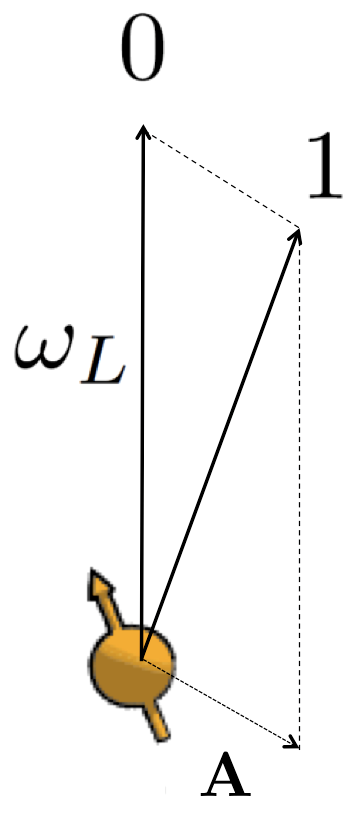
\includegraphics[keepaspectratio,width=0.2\textwidth,height=0.75\textheight]{./img/QuantizationAxis.png}
\caption{Flipping the electron spin from the  $m_s=0$ to the $m_s= -1$ state changes the quantization axis of $^{13}\mathrm{C}$ nuclear spins. For  $m_s=0$ spins precess about $\omega_L$. For  $m_s=-1$ spins precess about a distinct axis $\mathbf{\tilde{\omega}}=\mathbf{\omega_L} +\mathbf{A}$~\citep{Taminiau2012Detection}}
\label{fig:quantax}
\end{figure}


\section{Structure of a typical experiment}
Lorem ipsum dolor sit amet, consectetur adipisicing elit, sed do eiusmod
tempor incididunt ut labore et dolore magna aliqua. Ut enim ad minim veniam,
quis nostrud exercitation ullamco laboris nisi ut aliquip ex ea commodo
consequat. Duis aute irure dolor in reprehenderit in voluptate velit esse
cillum dolore eu fugiat nulla pariatur. Excepteur sint occaecat cupidatat non
proident, sunt in culpa qui officia deserunt mollit anim id est laborum.
